Data4Help Core is the central component of the system that connects all the other parts of the structure.

\begin{figure}[H]
	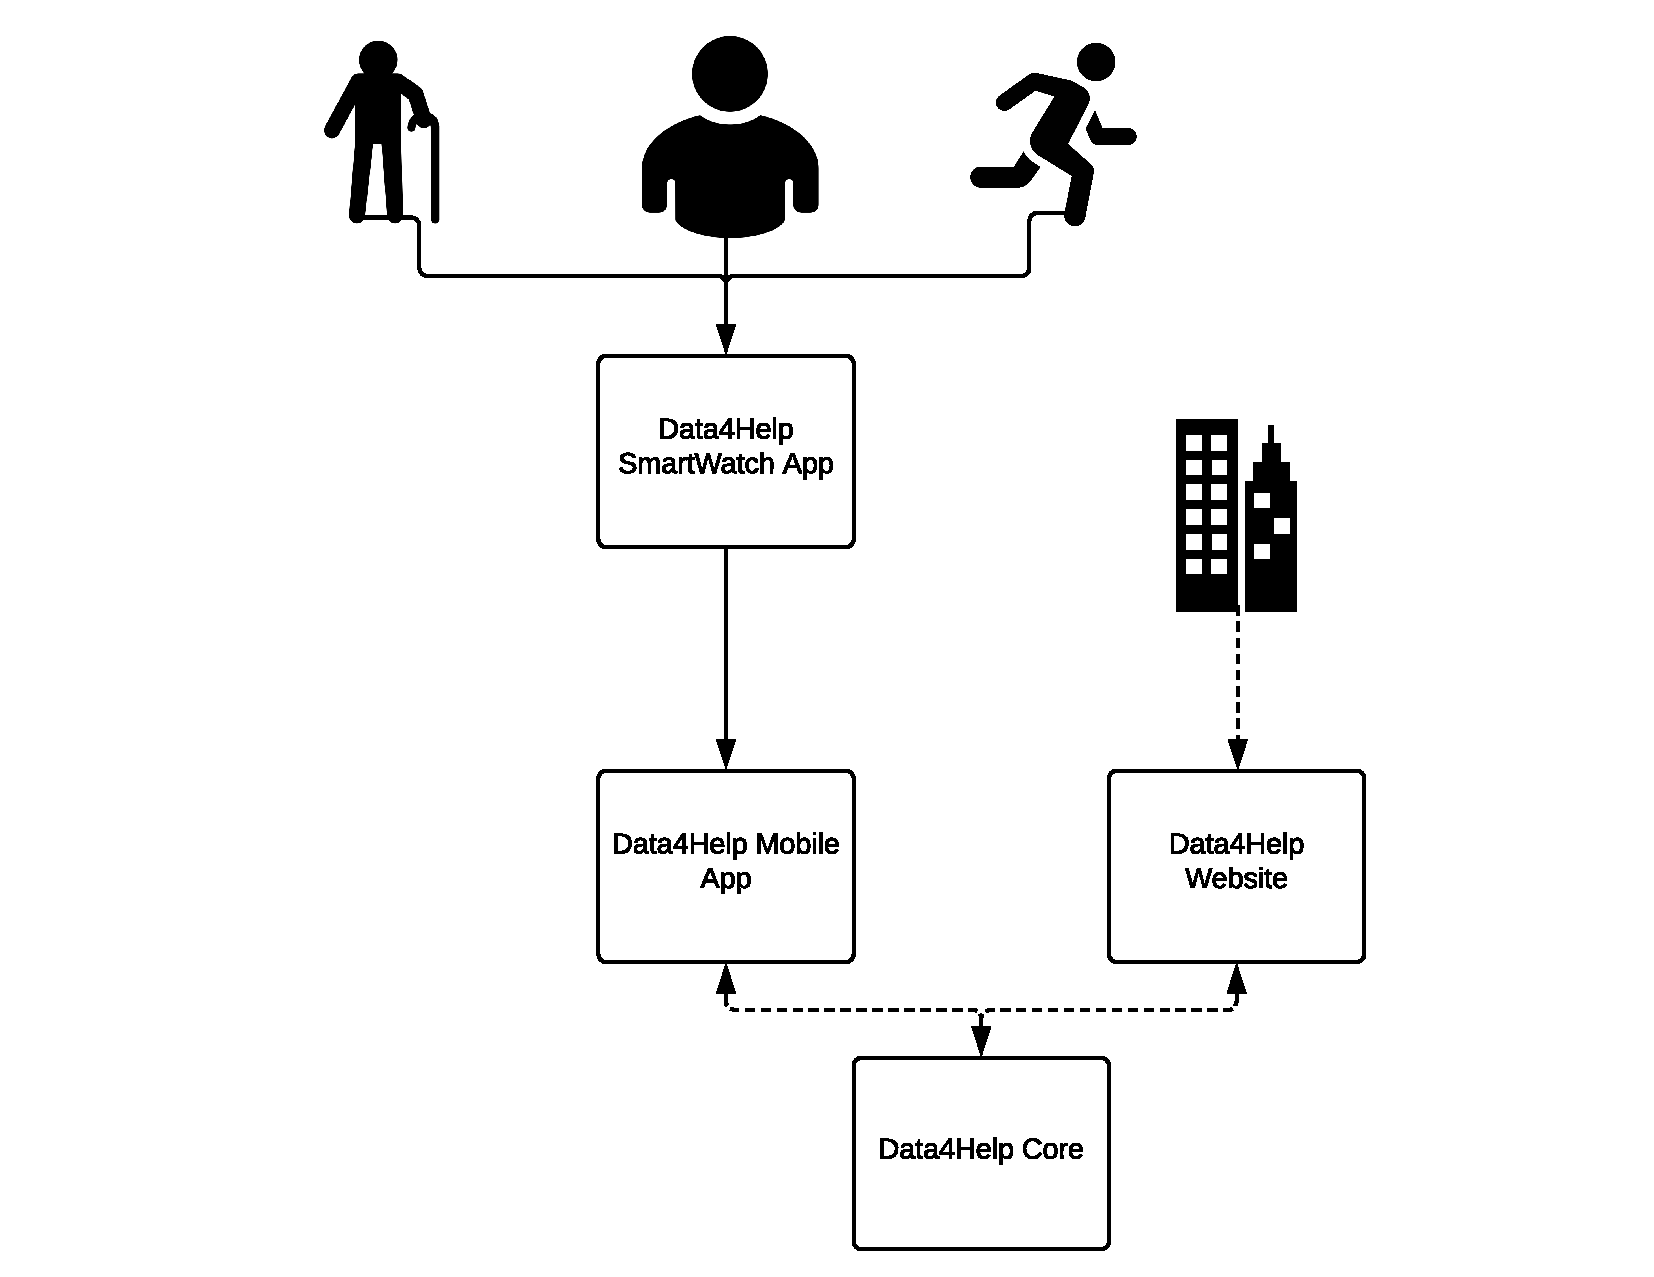
\includegraphics[width=\textwidth,height=\textheight,keepaspectratio]{assets/useflow.pdf}
	\caption{Use flow diagram}
	\label{fig:useflow}
\end{figure}

The Smartwatch App should be directly connected to the Mobile App to acquire data and let them be shown in the smartphone. In turn, the Mobile App has to communicate with the Data4Help Core that will register the data of the user. The Data4Help Website should communicate with the Data4Help Core as well in order to query directly on the company database.
\newline

\subsubsection{State charts}

\paragraph{Query request}
The following state diagram shows the state of a Query made by a Company. As soon as the Query is made from a registered Company, it goes into the \textit{Waiting for Data} state. Then the Query can either be removed by the Company or new data can satisfy the Query. In the latter case the query goes into the \textit{Check Active Subscription} state. If a Subscription is active, the Query goes into the \textit{New Data Available} state, otherwise it goes into \textit{Payment Request}. If the transaction is accepted, the new state is \textit{New Data Available}, otherwise goes into \textit{Payment Failed State}, until the payment method is updated.

\begin{figure}[H]
	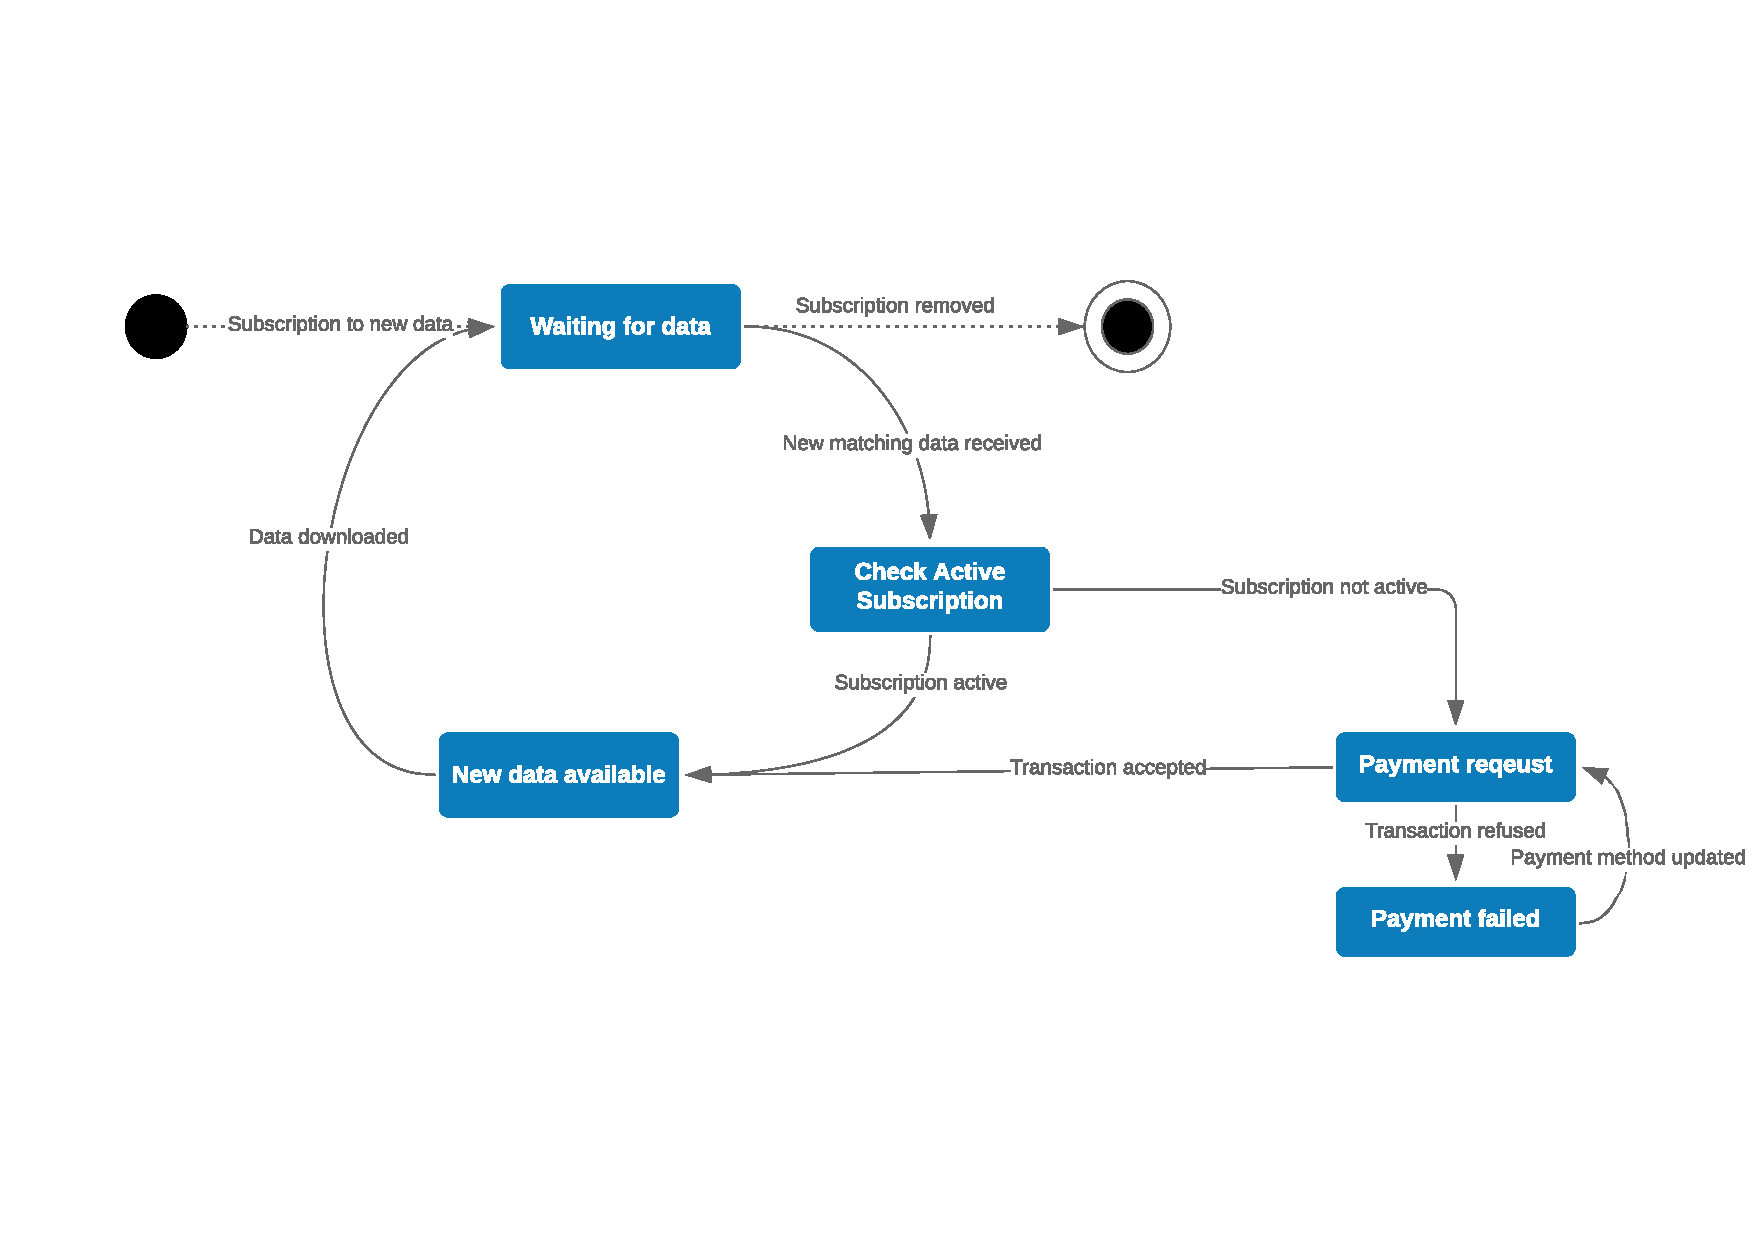
\includegraphics[width=\textwidth,height=\textheight,keepaspectratio]{assets/Data_request.pdf}
	\caption{Data request state diagram}
	\label{fig:DataRequest}
\end{figure}




\paragraph{Individuals data query}
When a Company creates a Query, it goes into the \textit{Check Active Subscription} state. If the subscription to make individual queries is active, the system asks to the user for the permission. If the permission is granted, the Query goes into \textit{Company Subscribed} and the company can access user's data. If either the user denies the request or remove the permission to the company after having accepted the request, the Query is deleted.
If the subscription is not active, the new state is \textit{Payment Request}. If the transaction is accepted then the new state is \textit{Check Active Subscription}, otherwise the transaction is refused, the new state is \textit{Payment Failed} and the Query waits until the user update his payment method.

\begin{figure}[H]
	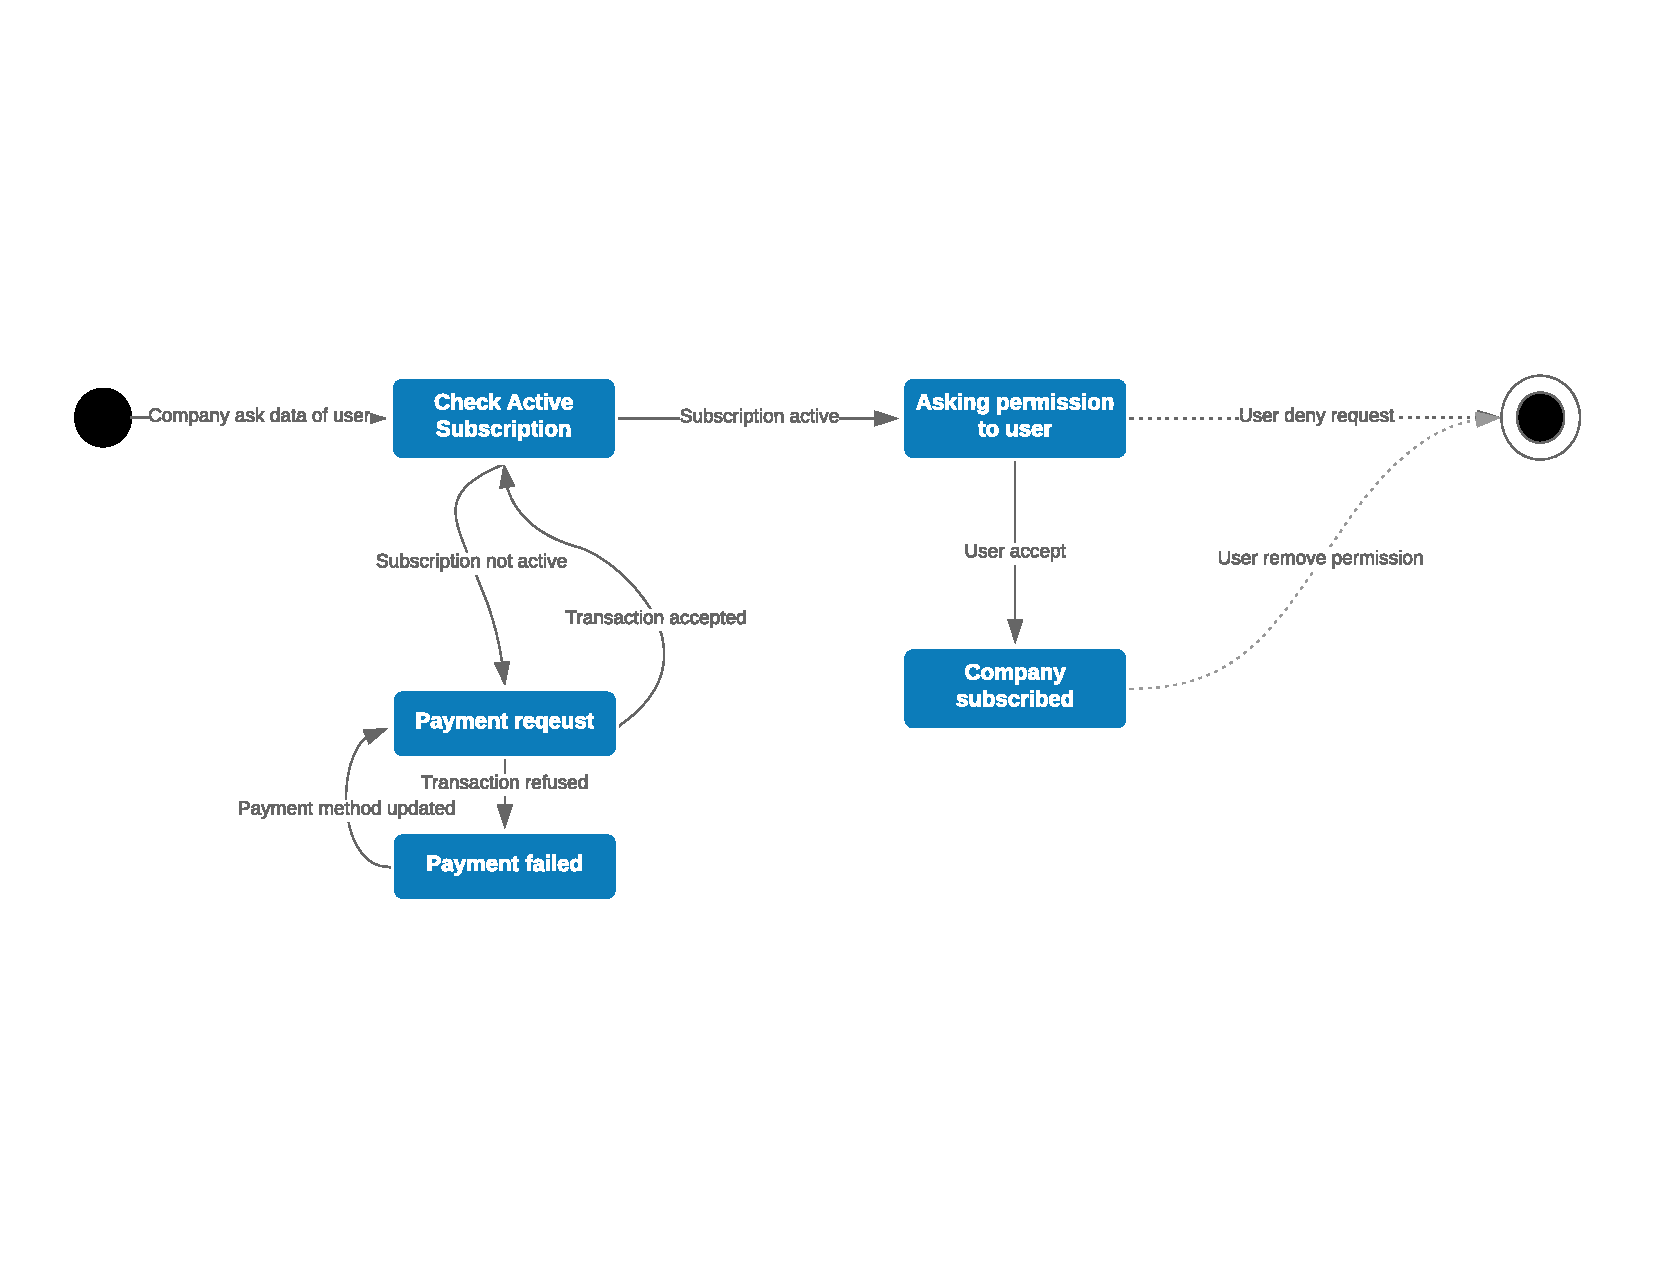
\includegraphics[width=\textwidth,height=\textheight,keepaspectratio]{assets/IndividualRequest.pdf}
	\caption{Individual request state diagram}
	\label{fig:IndividualRequest}
\end{figure}

\newpage
\subsection{Class diagram}
\begin{figure}[H]
	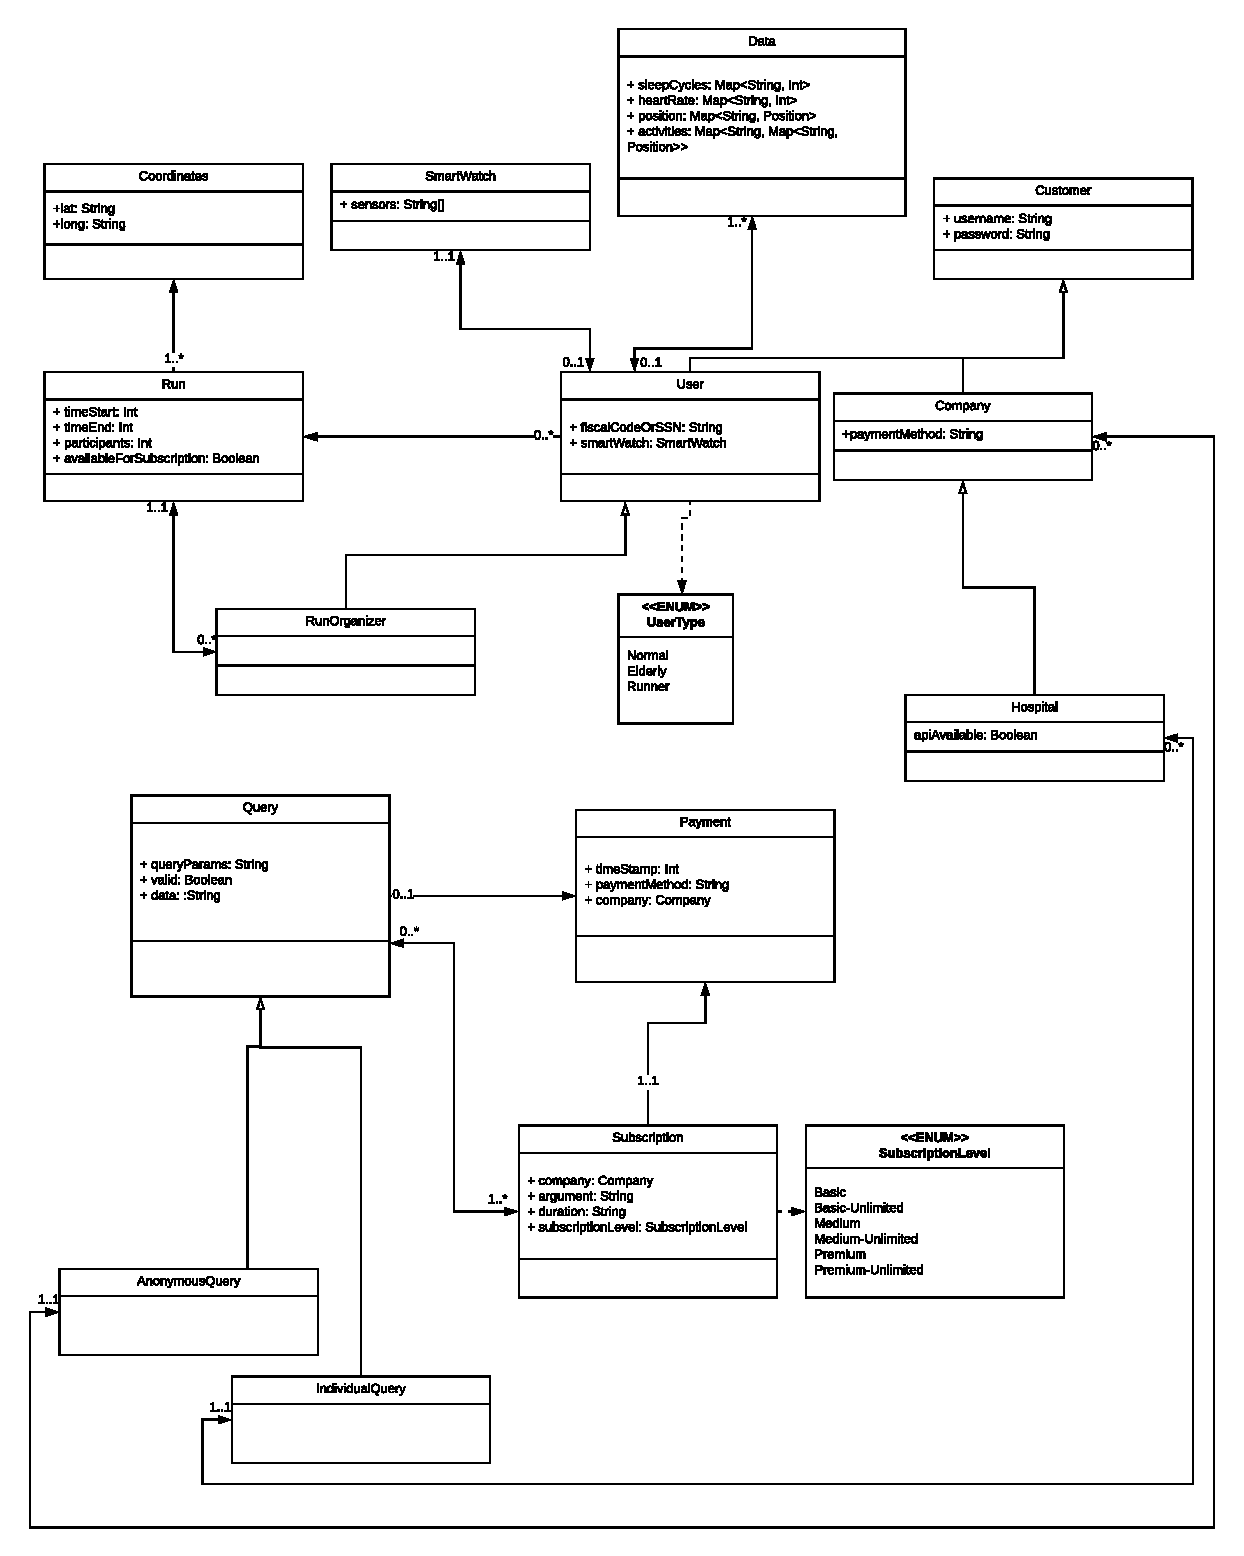
\includegraphics[width=\textwidth,height=\textheight,keepaspectratio]{assets/UML.pdf}
	\caption{Class diagram}
	\label{fig:ClassDiagram}
\end{figure}